\documentclass{report}
\usepackage[utf8]{inputenc}

%----- Configuración del estilo del documento------%
\usepackage{epsfig,graphicx}
\usepackage[left=2.5cm,right=2.5cm,top=1.8cm,bottom=2.3cm]{geometry}
%------ Paquetes matematicos --------%
\usepackage{amsmath}
\usepackage{amssymb}
\usepackage{amsthm}
\usepackage{amsmath}
\usepackage{tabularx}
\usepackage{fancyhdr}
\usepackage{lastpage}
\usepackage{verbatim}
\usepackage[shortlabels]{enumitem}
\usepackage{venndiagram}
\usetikzlibrary{shapes.geometric}
\usepackage{cancel}
\usepackage{hyperref}
\usepackage[T1]{fontenc}
\usepackage[spanish,es-nodecimaldot,es-tabla]{babel}
\usepackage{csquotes}
\usepackage{graphicx}
\usepackage{tocloft}
\graphicspath{{./figs/}}
\usepackage{setspace}
\usepackage{xcolor}


\usepackage[backend=biber]{biblatex}
\addbibresource{resources/referencias/referencias.bib}

\begin{document}
	
	\begin{titlepage}
	\thispagestyle{empty}
	\begin{minipage}[c][0.17\textheight][c]{0.25\textwidth}
		\begin{center}
			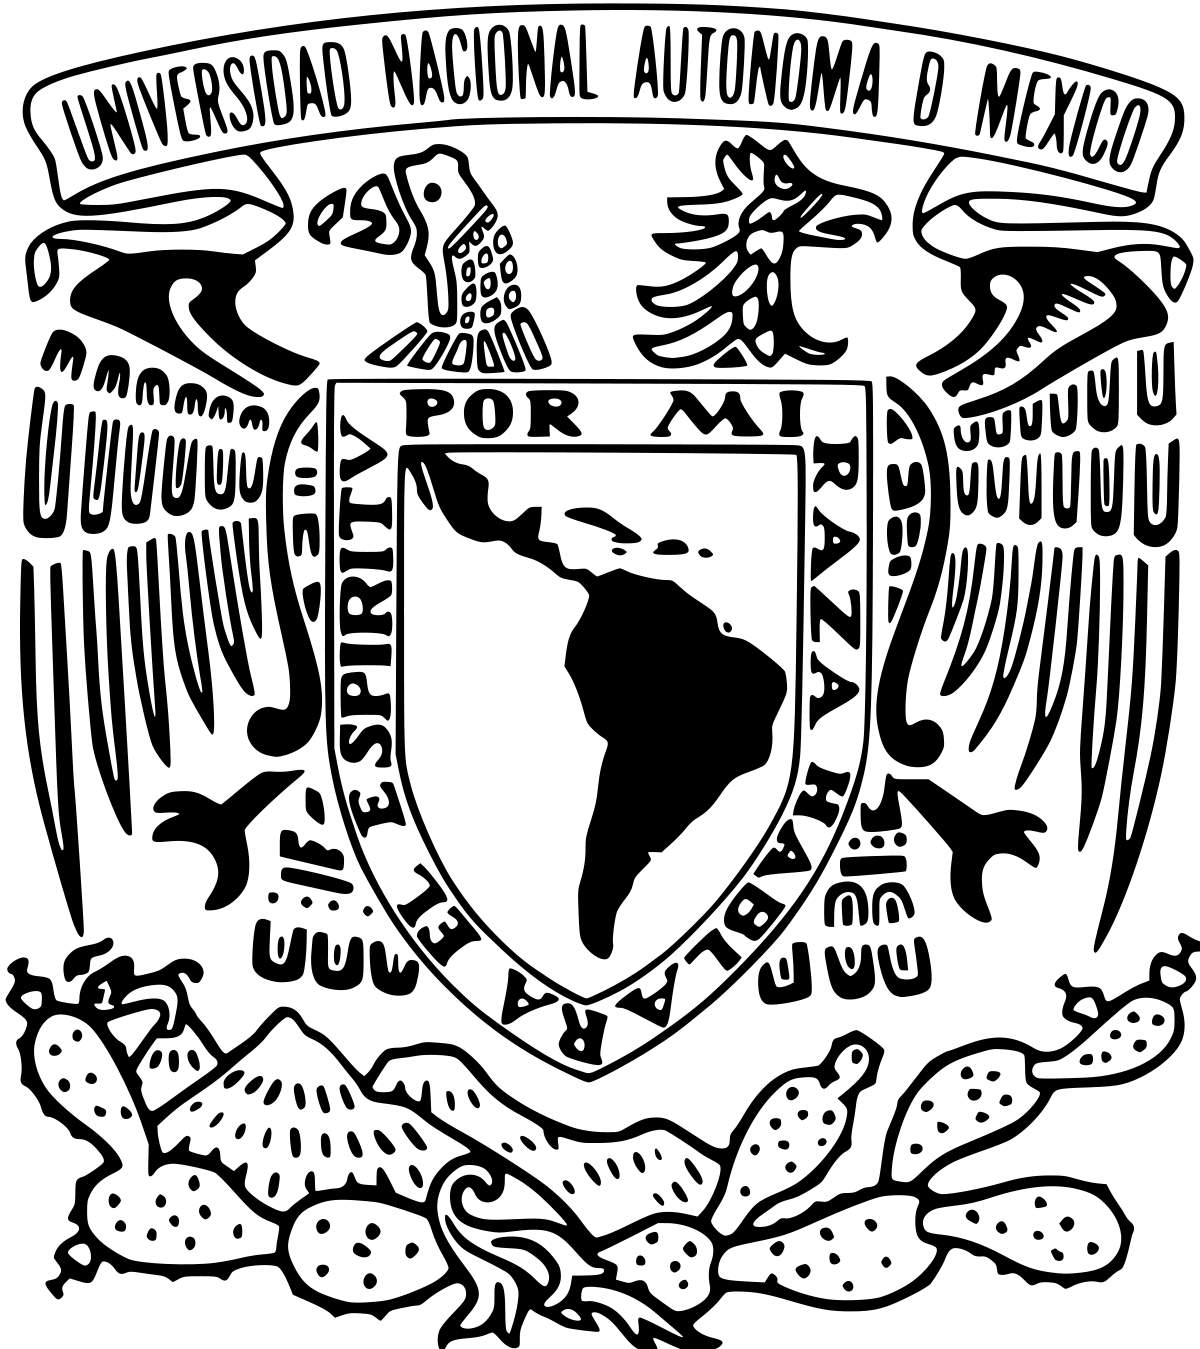
\includegraphics[width=3.5cm, height=3.5cm]{resources/Logo_UNAM.png}
		\end{center}
	\end{minipage}
	\begin{minipage}[c][0.195\textheight][t]{0.75\textwidth}
		\begin{center}
			\vspace{0.3cm}
			\textsc{\large Universidad Nacional Aut\'onoma de M\'exico}\\[0.5cm]
			\vspace{0.3cm}
			\hrule height2.5pt
			\vspace{.2cm}
			\hrule height1pt
			\vspace{.8cm}
			\textsc{Facultad de Ciencias}\\[0.5cm] %
		\end{center}
	\end{minipage}
	
	\begin{minipage}[c][0.81\textheight][t]{0.25\textwidth}
		\vspace*{5mm}
		\begin{center}
			\hskip2.0mm
			\vrule width1pt height13cm 
			\vspace{5mm}
			\hskip2pt
			\vrule width2.5pt height13cm
			\hskip2mm
			\vrule width1pt height13cm \\
			\vspace{5mm}
			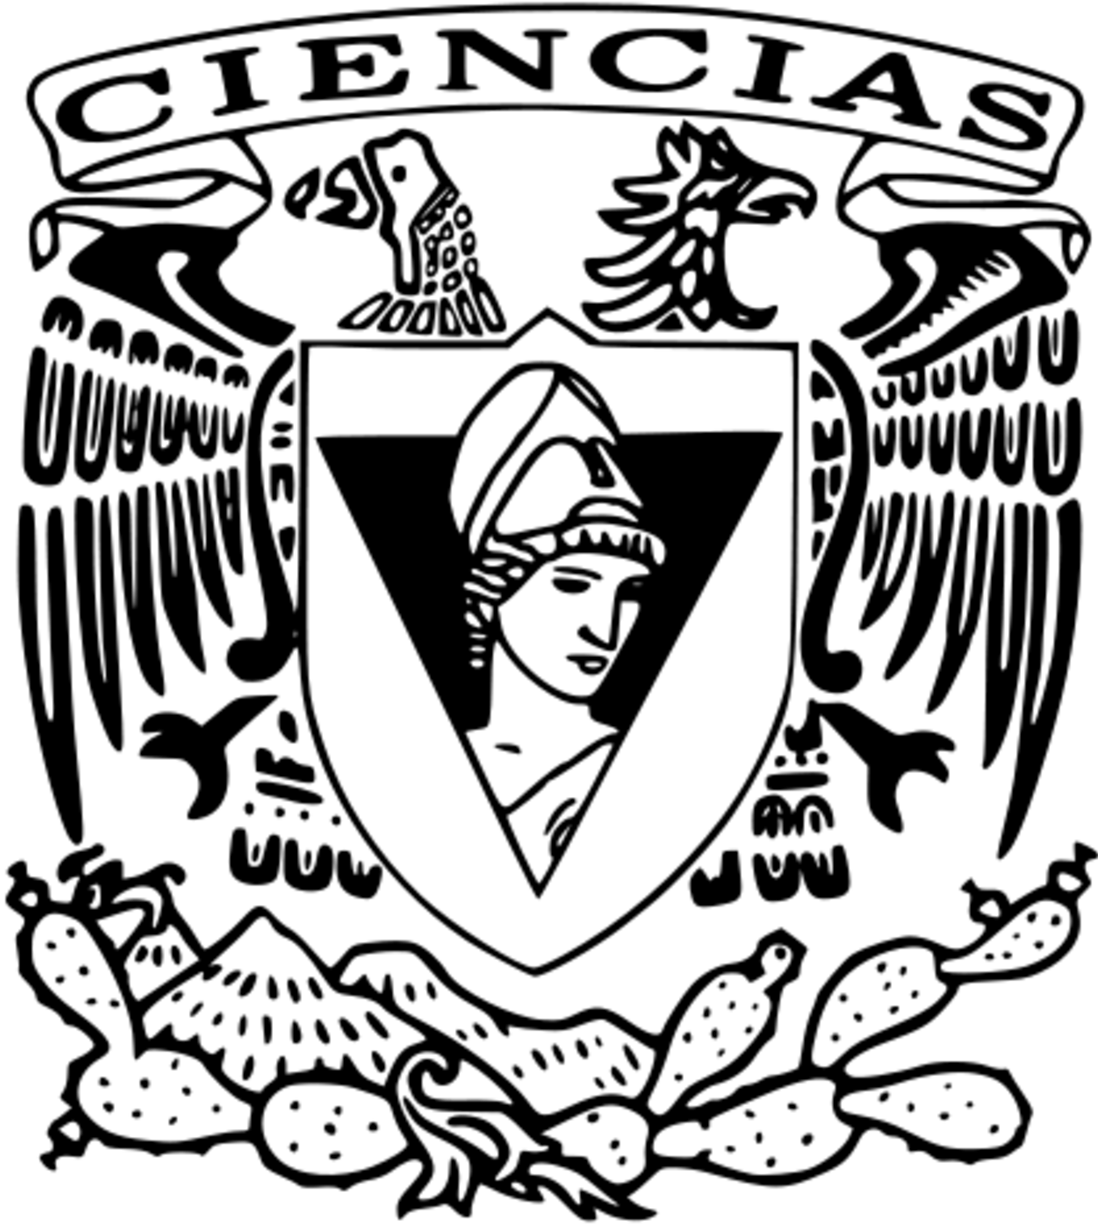
\includegraphics[height=4.0cm]{resources/Logo_FC.png}
		\end{center}
	\end{minipage}
	\begin{minipage}[c][0.81\textheight][t]{0.75\textwidth}
		\begin{center}
			\vspace{1cm}
			
			{\large\scshape Fundamentos de Bases de Datos - 7094}\\[.2in]
			
			\vspace{2cm}            
			
			\textsc{\LARGE \textbf{T}\hspace{1cm}\textbf{A}\hspace{1cm}\textbf{R}\hspace{1cm}\textbf{E}\hspace{1cm}\textbf{A}\hspace{1cm}\hspace{1cm}\textbf{4}}\\[2cm]
			\textsc{\Large{Equipo:}\normalsize \\
                \vspace{.3cm}
				\textbf{Del Monte Ortega Maryam Michelle - 320083527 \\
                \vspace{.2cm}
				\href{https://github.com/JuanSosaCiencias}{\textcolor{blue}{Sosa Romo Juan Mario - 320051926}} \\
                \vspace{.2cm}
				Castillo Hernández Antonio - 320017438 \\
                \vspace{.2cm}
                Erik Eduardo Gómez López - 320258211 \\
                \vspace{.2cm}
                Julio César Islas Espino - 320340594}}\\[0.5cm]     
			
			\textsc{{Fecha de entrega: \\ \textbf{10 de Octubre de 2024}}}\\[0.5cm]        
			
			\textsc{{Profesor: \\ \textbf{M. en I. Gerardo Avilés Rosas}}}\\[0.5cm]  
			
			\textsc{Ayudantes: \\ \textbf{Luis Enrique García Gómez \\ Kevin Jair Torres Valencia \\ Ricardo Badillo Macías \\ Rocío Aylin Huerta González
			} }
			
			
			\vspace{0.5cm}
		\end{center}
	\end{minipage}
\end{titlepage}

	
    % Parte 1
	\begin{center}
		\section*{\LARGE{Tarea 2}}
	\end{center}

    \begin{center}
        \LARGE{\textbf{Conceptos del Modelo Entidad – Relación}}\\
    \end{center}
    \normalsize

    \begin{enumerate}[label=\alph*.]
        \item \textbf{Dos compañías con el nombre ‘Panaphonics’ podrían existir al mismo tiempo.}\vspace{.3cm}

\begin{quote}
    Voy a asumir que la relación \textbf{Proyecto} es donde se pondría el nombre de la compañía (que no se que tanto sentido tenga hacer esto para el departamento de RH de una empresa pero bueno). Vemos que en esta relación el único atributo que no se puede repetir es \textbf{NumProyecto} pues es la clave primaria. Por lo tanto, si se puede tener dos compañías con el nombre ‘Panaphonics’ al mismo tiempo. \vspace{.2cm}

    Si se quisiera que solo existiera una compañía con el nombre ‘Panaphonics’ al mismo tiempo, se podría definir el atributo \textbf{NombreCompañía} como clave primaria o una llave primaria compuesta con el atributo \textbf{NumProyecto}.
\end{quote}
\vspace{.3cm}
        \item \textbf{Del inciso a) toma el MR que obtuviste para la cardinalidad M : N. Asume que los atributos a1, b y ab1 son de tipo
entero, mientras que a2, a3 y b1 son de tipo cadena. Supón que la relación A tiene 4 tuplas con los siguientes valores
(2,’ww’,’a’), (4,’xx’,’b’), (6,’yy’,’c’), (8,’zz’,’d’) y la relación B tiene 5 tuplas identificadas por
los valores 17, 27, 37, 47, 57. Los incisos que se presentan a continuación, representan un conjunto de tuplas
a insertar (en ese orden) en la relación AB, indica cuál conjunto se puede insertar completamente en dicha relación.
Justifica tu respuesta en cada caso.}\vspace{.3cm}

\begin{enumerate}
    \item (8,’zz’,17,5); (6,’yy’,57,10); (4,’xx’,27,15); (2,’ww’,37,20); (4,’xx’,27,15)
    
    Podemos insertar (8,’zz’,17,5); (6,’yy’,57,10); (4,’xx’,27,15); (2,’ww’,37,20) y ya, insertar \textbf{otra vez} (4,’xx’,27,15) es innecesario ya que existiría más de una tupla con la misma llave.

    \item (17,’zz’,2,’m’); (27,’yy’,4,’n’); (37,’xx’,6,’o’); (47,’ww’,8,’p’); (57,’zz’,4,’q’)
    
    Ninguna se puede insertar ya que \textbf{ab1} es de tipo entero según las especificaciones y para este conjunto de tuplas, en todas se representa a \textbf{ab1} como cadena o caracter. 

    \item (2,’a’,17,23); (4,’b’,27,24); (6,’c’,37,25); (8,’d’,47,26); (2,’a’,57,27)
    
    Todas se pueden insertar, ya que los tipos de datos están correctos y no hay tuplas duplicadas ya que todas tienen más de un atributo distinto. 

    \item (2,’ww’,57,’a’); (4,’xx’,37,’b’); (6,’yy’,17,’c’); (8,’zz’,37,’d’); (4,’xx’,47,’a’)
    
    Nuevamente no podemos insertar ninguna ya que \textbf{ab1} es de tipo entero y se le pasan cadenas. 
\end{enumerate}

\vspace{.5cm}

        \item \textbf{Del inciso a) toma como base el MR que obtuviste para la cardinalidad 1 : N. Los incisos que se presentan a
continuación representan un conjunto de tuplas a insertar (en ese orden) en la relación B, indica cuál conjunto se
puede insertar completamente en dicha relación. Justifica tu respuesta en cada caso.}\vspace{.3cm}

\begin{enumerate}
    \item (2,’f’,57,’zz’); (4,’g’,47,’yy’); (6,’h’,37,’xx’); (8,’i’,27,’ww’); (2,’j’,17,’yy’)
    \item (57,8,’zz’,’f’); (47,6,’yy’,’g’); (37,4,’xx’,’h’); (27,2,’ww’,’i’); (17,6,’yy’,’j’)
    \item (57,’f’,8,’zz’); (47,’g’,6,’yy’); (37,’h’,4,’xx’); (27,’i’,2,’ww’); (17,’j’,6,’yy’)
    \item (57,’f’,8,’a’); (47,’g’,6,’b’); (37,’h’,4,’c’); (27,’i’,2,’d’); (17,’j’,6,’c’)
\end{enumerate}

\vspace{.5cm}

Tomando como base el modelo relacional obtenido para la relación 1:N del inciso a), procederemos a analizar cada conjunto de tuplas para determinar cuál de ellos se puede insertar completamente en la relación \texttt{B}. \\

\begin{enumerate}
    \item \textbf{(2,’f’,57,’zz’); (4,’g’,47,’yy’); (6,’h’,37,’xx’); (8,’i’,27,’ww’); (2,’j’,17,’yy’)} \\
    
    En este caso, los valores de \texttt{b} (57, 47, 37, 27, 17) son todos únicos, por lo que no hay problemas con la clave primaria en \texttt{B}. Además, las combinaciones de \texttt{a1} y \texttt{a2} (\texttt{(2,'zz')}, \texttt{(4,'yy')}, \texttt{(6,'xx')}, \texttt{(8,'ww')}, \texttt{(2,'yy')}) no generan conflictos en términos de las claves foráneas. Si estas combinaciones existen en la tabla \texttt{A}, se pueden insertar sin problemas. \\
    
    $\therefore$ El conjunto de tuplas se puede insertar completamente. \\

    \item \textbf{(57,8,’zz’,’f’); (47,6,’yy’,’g’); (37,4,’xx’,’h’); (27,2,’ww’,’i’); (17,6,’yy’,’j’)} \\
    
    Los valores de \texttt{b} (57, 47, 37, 27, 17) son diferentes, por lo que no hay conflictos con la clave primaria en \texttt{B}. Las combinaciones de \texttt{a1} y \texttt{a2} (\texttt{(8,'zz')}, \texttt{(6,'yy')}, \texttt{(4,'xx')}, \texttt{(2,'ww')}, \texttt{(6,'yy')}) muestran una repetición de \texttt{(6,'yy')}, pero mientras esa combinación sea válida en \texttt{A}, no debería haber problemas para insertar las tuplas en \texttt{B}. \\

    $\therefore$ El conjunto de tuplas se puede insertar completamente.\\

    \item \textbf{(57,’f’,8,’zz’); (47,’g’,6,’yy’); (37,’h’,4,’xx’); (27,’i’,2,’ww’); (17,’j’,6,’yy’)} \\
    
    En este conjunto, los valores de \texttt{b} (57, 47, 37, 27, 17) son únicos, lo cual es correcto para la clave primaria de \texttt{B}. Las combinaciones de \texttt{a1} y \texttt{a2} (\texttt{(8,'zz')}, \texttt{(6,'yy')}, \texttt{(4,'xx')}, \texttt{(2,'ww')}, \texttt{(6,'yy')}) incluyen una duplicación de \texttt{(6,'yy')}, pero si esta combinación es válida en \texttt{A}, no habría problemas para que las tuplas se inserten en \texttt{B}. \\

    $\therefore$ Este conjunto de tuplas se puede insertar completamente.

    \item \textbf{(57,’f’,8,’a’); (47,’g’,6,’b’); (37,’h’,4,’c’); (27,’i’,2,’d’); (17,’j’,6,’c’)} \\
    
    Aquí los valores de \texttt{b} (57, 47, 37, 27, 17) siguen siendo únicos, por lo que no hay conflicto con la clave primaria en \texttt{B}. Sin embargo, la combinación de \texttt{a1} y \texttt{a2} \texttt{(6,'c')} aparece en dos tuplas, lo cual es un problema, ya que \texttt{a1} y \texttt{a2} forman parte de la clave primaria compuesta en \texttt{A}. Esta duplicación no es válida, lo que viola la integridad referencial y, por lo tanto, no es posible insertar todas las tuplas. \\

    $\therefore$ Este conjunto de tuplas no se puede insertar completamente.
\end{enumerate}

        \item \textbf{Considera el mismo escenario del inciso b para las relaciones A y B. Toma como base el Modelo Relacional que
obtuviste para la cardinalidad 1:1. Supón que tu modelo tiene participación parcial de ambos lados. Propón un
conjunto de 4 tuplas que se pueda insertar en ab y un conjunto que no se pueda insertar (también de 4 tuplas).
Justifica tu respuesta en cada caso.}\vspace{.3cm}
\subsubsection*{Conjunto de 4 tuplas que se pueden insertar en \( AB \)}

Supongamos que las tuplas presentes en \( A \) y \( B \) son las siguientes:

\begin{itemize}
    \item \( A: (2, \text{'ww'}, \text{'a'}), (4, \text{'xx'}, \text{'b'}), (6, \text{'yy'}, \text{'c'}), (8, \text{'zz'}, \text{'d'}) \)
    \item \( B: (17, \text{'e'}), (27, \text{'f'}), (37, \text{'g'}), (47, \text{'h'}) \)
\end{itemize}

Propuestas de tuplas para \( AB \):

\begin{enumerate}
    \item (2, \text{'ww'}, 17, 10)
    \item (4, \text{'xx'}, 27, 20)
    \item (6, \text{'yy'}, 37, 30)
    \item (8, \text{'zz'}, 47, 40)
\end{enumerate}


Estas tuplas se pueden insertar porque:

\begin{itemize}
    \item Cada \( (a1, a2) \) de \( AB \) corresponde a una combinación válida de claves primarias de \( A \).
    \item Cada \( b \) en \( AB \) coincide con una clave primaria en \( B \).
    \item Las combinaciones de \( (a1, a2) \) y \( b \) son únicas, respetando la restricción de 1:1, sin repetir la asociación entre \( A \) y \( B \).
\end{itemize}

\subsubsection*{Conjunto de 4 tuplas que no se pueden insertar en \( AB \)}

\begin{enumerate}
    \item (2, \text{'ww'}, 17, 10)
    \item (2, \text{'ww'}, 27, 20)
    \item (4, \text{'xx'}, 27, 30)
    \item (4, \text{'xx'}, 47, 40)
\end{enumerate}


Estas tuplas no se pueden insertar debido a que:

\begin{itemize}
    \item Las primeras dos tuplas intentan asociar la misma tupla de \( A \) (\( 2, \text{'ww'} \)) con diferentes tuplas de \( B \) (17 y 27), violando la restricción de 1:1.
    \item Las últimas dos tuplas intentan asociar la misma tupla de \( A \) (\( 4, \text{'xx'} \)) con diferentes tuplas de \( B \) (27 y 47), lo cual también infringe la relación 1:1.
    \item La relación 1:1 implica que una tupla de \( A \) solo puede estar asociada con una única tupla de \( B \) y viceversa, y estas tuplas propuestas intentan establecer múltiples asociaciones.
\end{itemize}

        \item 
Explica el concepto de categorías (herencia múltiple) en el modelo E-R y proporciona dos ejemplos de la vida real en donde se aplique este concepto.

Las \textbf{categorías} (o herencia múltiple) en el modelo E-R permite que una entidad pueda heredar sus atributos a otras entidades, donde la entidad hija \textbf{(subtipo)}, hereda los atributos y relaciones de una o múltiples entidades padres \textbf{(supertipo)}. Esto significa que la entidad hija se relaciona con varias entidades padres, combinando sus características.

Ejemplos:
\begin{itemize}
    \item \textbf{Ejemplo 1:}
    \begin{itemize}
        \item \textbf{Supertipo: } Empleado y Consultor
        \item \textbf{Subtipo:} Empleado-Consultor
        
    \begin{itemize}
        \item La entidad \textbf{Empleado} contiene atributos como 'Número de empleado', 'Salario', 'Departamento'.
        \item La entidad \textbf{Consultor} tiene atributos como 'Número de proyecto', 'Tarifa por hora', 'Fecha de finalización'.
        \item La entidad \textbf{Empleado-Consultor} hereda atributos tanto de \textbf{Empleado} como de \textbf{Consultor}, y puede tener atributos adicionales como 'Horas dedicadas como consultor'. Esta entidad representa a un trabajador que es tanto un empleado fijo de una empresa como un consultor en proyectos específicos.
    \end{itemize}
    \end{itemize}

    \item \textbf{Ejemplo 2:}
    \begin{itemize}
         \item \textbf{Supertipo:} Persona
        \item \textbf{Subtipo:} Estudiante y Profesor
        
    \begin{itemize}
        \item La entidad \textbf{Persona} contiene atributos comunes como 'Nombre', 'Edad" y 'Dirección'.
        \item Las entidades hijas \textbf{Estudiante} y \textbf{Profesor} heredan esos atributos comunes, pero tienen atributos adicionales específicos:
        \begin{itemize}
            \item \textbf{Estudiante:} 'Número de matrícula', 'Carrera'.
            \item \textbf{Profesor:} 'Número de empleado', 'Departamento'.
        \end{itemize}
    \end{itemize}
    \end{itemize}
\end{itemize}

    \end{enumerate}

    % Parte 2  
    \begin{center}
        \LARGE{\textbf{Entendiendo el Modelo Entidad – Relación}}\\
    \end{center}
    \normalsize

    \begin{enumerate}%[label=\alph*.]
        \item \textbf{Entrenadores y Atletas, que compartan el apellido y que se encuentren participando en la misma disciplina.
Deberan ordenar la información a partir del apellido paterno.}\vspace{.3cm}
        \item \section*{Consulta 2: Cantidad de asistentes y ganancias por disciplina y localidad}

\subsection*{Descripción}
Esta consulta calcula cuántas personas asistieron y cuánto dinero se ganó en cada disciplina y localidad. Es útil para evaluar el éxito financiero y la popularidad de los eventos en distintas áreas.

\textbf{SQL}

\begin{verbatim}
SELECT 
    d.NombreDisciplina,
    l.NombreLocalidad,
    SUM(e.Precio) AS GananciasTotales,
    COUNT(ce.IDCliente) AS CantidadAsistentes
FROM 
    Evento e
JOIN 
    Disciplina d ON e.IDDisciplina = d.IDDisciplina
JOIN 
    Localidad l ON e.NombreLocalidad = l.NombreLocalidad AND e.IDDisciplina = l.IDDisciplina
JOIN 
    CompraEntrada ce ON e.IDEvento = ce.IDEvento
GROUP BY 
    d.NombreDisciplina, l.NombreLocalidad
ORDER BY 
    CantidadAsistentes DESC;
\end{verbatim}

\begin{center}
    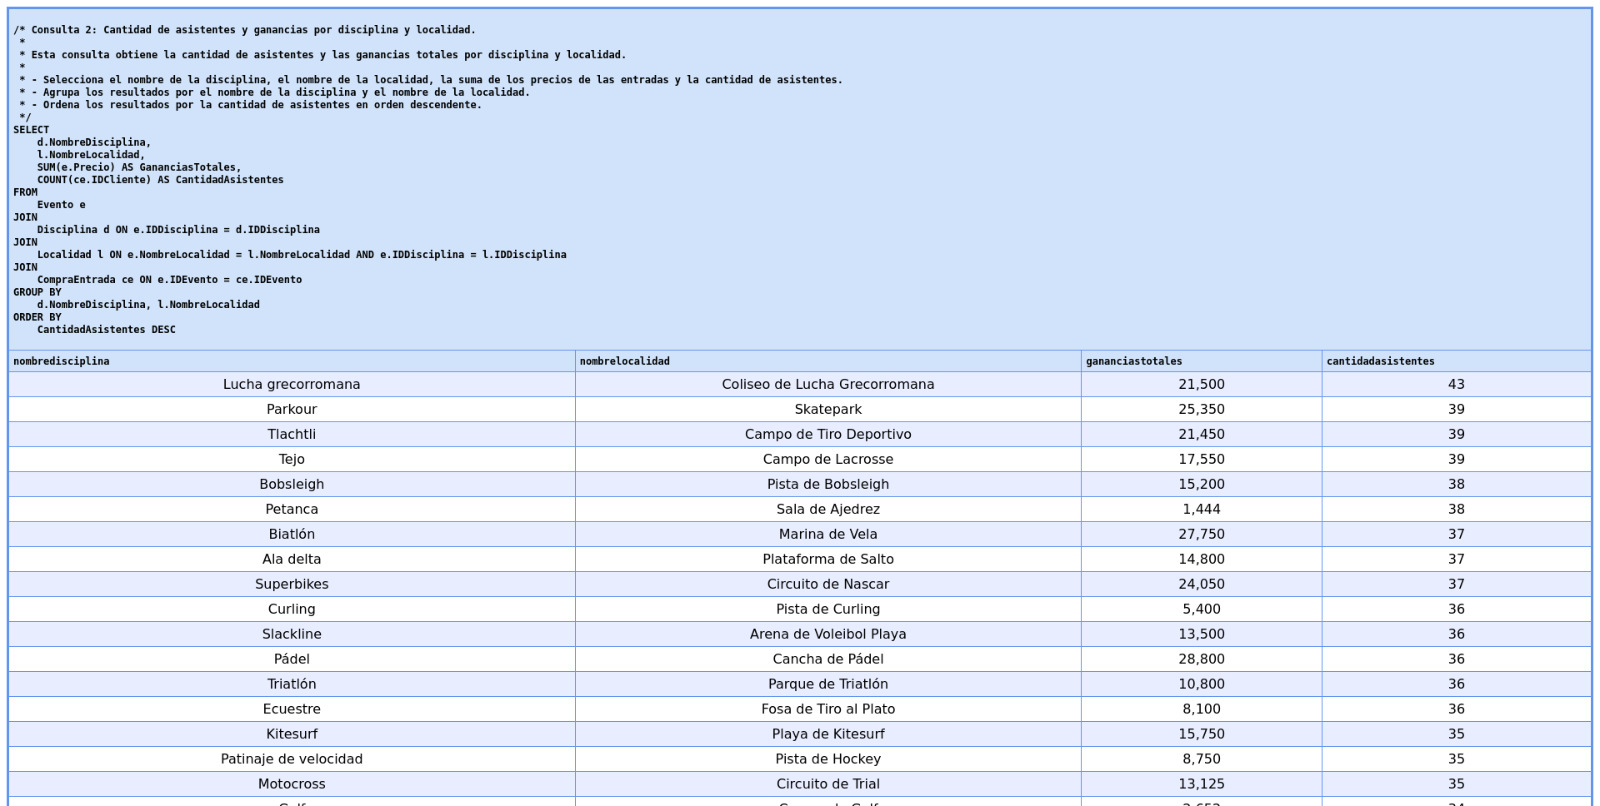
\includegraphics[width=16.5cm]{../resources/Chapters/Consultas/Imagenes/Consulta2.jpeg} 
    
   Consulta 2. Cantidad de asistentes y ganancias por disciplina y localidad. 
\end{center}

\textbf{Desglose de la consulta}

\begin{itemize}
   \item \textbf{Selección de columnas (\texttt{SELECT})}:
   \begin{itemize}
       \item Se seleccionan las siguientes columnas:
       \begin{itemize}
           \item \texttt{d.NombreDisciplina}: Nombre de la disciplina.
           \item \texttt{l.NombreLocalidad}: Nombre de la localidad.
           \item \texttt{SUM(e.Precio)}: Suma de los precios de las entradas, denominada \texttt{GananciasTotales}.
           \item \texttt{COUNT(ce.IDCliente)}: Cuenta la cantidad de asistentes, denominada \texttt{CantidadAsistentes}.
       \end{itemize}
   \end{itemize}
   
   \item \textbf{Tablas involucradas (\texttt{FROM} y \texttt{JOIN})}:
   \begin{itemize}
       \item La consulta utiliza cuatro tablas:
       \begin{itemize}
           \item \texttt{Evento (e)}: Contiene la información de los eventos.
           \item \texttt{Disciplina (d)}: Contiene la información de las disciplinas.
           \item \texttt{Localidad (l)}: Contiene la información de las localidades.
           \item \texttt{CompraEntrada (ce)}: Contiene la información de las entradas compradas.
       \end{itemize}
       \item Se realizan \texttt{JOINs} entre las tablas para relacionar los eventos con las disciplinas, localidades y entradas compradas.
   \end{itemize}
   
   \item \textbf{Agrupación de resultados (\texttt{GROUP BY})}:
   \begin{itemize}
       \item Para calcular la cantidad de asistentes y las ganancias por disciplina y localidad, se agrupan los datos según las columnas:
       \begin{itemize}
           \item \texttt{d.NombreDisciplina}, \texttt{l.NombreLocalidad}.
       \end{itemize}
       \item Esto garantiza que se genere un registro único por cada combinación de disciplina y localidad.
   \end{itemize}
   
   \item \textbf{Ordenamiento de resultados (\texttt{ORDER BY})}:
   \begin{itemize}
       \item Los resultados se ordenan por la columna \texttt{CantidadAsistentes} en orden descendente (\texttt{DESC}), de modo que las combinaciones de disciplina y localidad con más asistentes aparezcan primero.
   \end{itemize}
\end{itemize}

\textbf{Análisis detallado}

\begin{enumerate}
   \item \textbf{Relación entre tablas:}
   \begin{itemize}
       \item La consulta asume que existe una relación directa entre las tablas \texttt{Evento}, \texttt{Disciplina}, \texttt{Localidad} y \texttt{CompraEntrada} a través de las claves foráneas.
       \item Esto implica que:
       \begin{itemize}
           \item Cada evento está asociado con una disciplina y una localidad.
           \item Cada entrada comprada está asociada con un evento.
       \end{itemize}
   \end{itemize}
   
   \item \textbf{Uso de funciones agregadas \texttt{SUM} y \texttt{COUNT}:}
   \begin{itemize}
       \item La función \texttt{SUM(e.Precio)} calcula las ganancias totales generadas por las entradas vendidas para cada combinación de disciplina y localidad.
       \item La función \texttt{COUNT(ce.IDCliente)} cuenta el número de asistentes para cada combinación de disciplina y localidad.
   \end{itemize}
   
   \item \textbf{Agrupación por disciplina y localidad:}
   \begin{itemize}
       \item El uso de \texttt{GROUP BY} permite agrupar los registros por disciplina y localidad, asegurando que las ganancias y la cantidad de asistentes se calculen correctamente para cada combinación.
   \end{itemize}
   
   \item \textbf{Ordenamiento:}
   \begin{itemize}
       \item El orden descendente por \texttt{CantidadAsistentes} facilita la identificación de las combinaciones de disciplina y localidad con mayor número de asistentes.
   \end{itemize}
\end{enumerate}

\textbf{Consideraciones}

\begin{itemize}
   \item \textbf{Empates en la cantidad de asistentes:}
   \begin{itemize}
       \item Si varias combinaciones de disciplina y localidad tienen la misma cantidad de asistentes, el orden relativo entre ellas no está definido. Para resolver esto, se podría agregar un criterio adicional en el \texttt{ORDER BY}, como las ganancias totales.
   \end{itemize}
\end{itemize}

        \item \textbf{Atletas que hayan participado en más de 1 disciplina.}\vspace{.3cm}
        \item 
Cómo modificarías el diagrama de la figura a) para representar las siguientes restricciones:\\
Un alumno no puede tomar clase en más de una materia con el mismo profesor. Una materia no puede ser
impartida por más de un profesor.

No es necesario realizar alguna modificación, pues la cardinalidad uno a uno que tiene el diagrama implica que un alumno no puede estar relacionado con el mismo profesor en más de una materia, y del mismo modo una materia no puede ser impartida por más de un profesor en la relación, por lo que el diagrama ya cumple con ambas restricciones.

        \item \begin{center}
    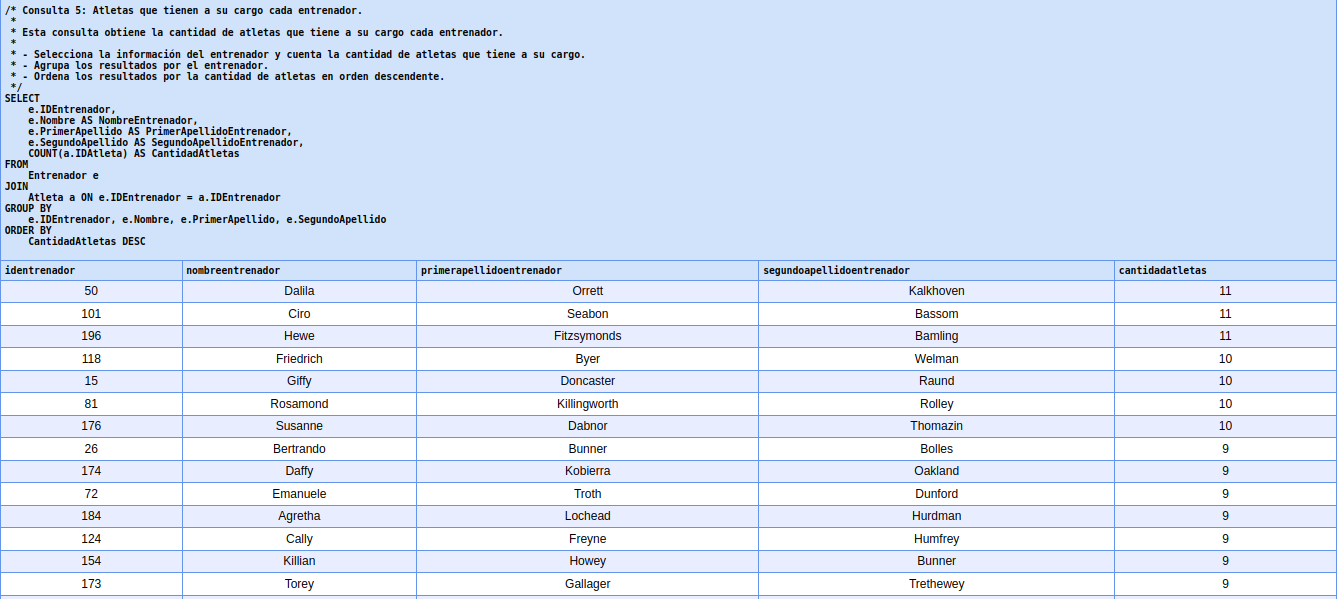
\includegraphics[width=16.5cm]{../resources/Chapters/Consultas/Imagenes/Consulta5.png} 
    
   Consulta 5. Atletas que tienen a su cargo cada entrenador. 
\end{center}

\textbf{Propósito de la consulta}

La consulta tiene como objetivo obtener un listado de entrenadores junto con la cantidad de atletas que tienen a su cargo. Esto es útil para entender la distribución de atletas entre los entrenadores y detectar posibles desequilibrios en la asignación de recursos.

\textbf{Desglose de la consulta}

\begin{itemize}
   \item \textbf{Selección de columnas (\texttt{SELECT})}:
   \begin{itemize}
       \item Se seleccionan las siguientes columnas del entrenador:
       \begin{itemize}
           \item \texttt{e.IDEntrenador}: Identificador único del entrenador.
           \item \texttt{e.Nombre}: Nombre del entrenador.
           \item \texttt{e.PrimerApellido}: Primer apellido del entrenador.
           \item \texttt{e.SegundoApellido}: Segundo apellido del entrenador.
       \end{itemize}
       \item Se utiliza la función agregada \texttt{COUNT(a.IDAtleta)} para contar cuántos atletas están asociados con cada entrenador. Esta columna se denomina \texttt{CantidadAtletas}.
   \end{itemize}
   
   \item \textbf{Tablas involucradas (\texttt{FROM} y \texttt{JOIN})}:
   \begin{itemize}
       \item La consulta utiliza dos tablas:
       \begin{itemize}
           \item \texttt{Entrenador (e)}: Contiene la información de los entrenadores.
           \item \texttt{Atleta (a)}: Contiene la información de los atletas.
       \end{itemize}
       \item Se realiza un \texttt{JOIN} entre ambas tablas utilizando la relación \texttt{e.IDEntrenador = a.IDEntrenador}. Esto asegura que solo se consideren los atletas que están asignados a un entrenador.
   \end{itemize}
   
   \item \textbf{Agrupación de resultados (\texttt{GROUP BY})}:
   \begin{itemize}
       \item Para calcular la cantidad de atletas por entrenador, se agrupan los datos según las columnas únicas del entrenador:
       \begin{itemize}
           \item \texttt{e.IDEntrenador}, \texttt{e.Nombre}, \texttt{e.PrimerApellido}, \texttt{e.SegundoApellido}.
       \end{itemize}
       \item Esto garantiza que se genere un registro único por cada entrenador.
   \end{itemize}
   
   \item \textbf{Ordenamiento de resultados (\texttt{ORDER BY})}:
   \begin{itemize}
       \item Los resultados se ordenan por la columna \texttt{CantidadAtletas} en orden descendente (\texttt{DESC}), de modo que los entrenadores con más atletas aparezcan primero.
   \end{itemize}
\end{itemize}

\textbf{Análisis detallado}

\begin{enumerate}
   \item \textbf{Relación entre tablas:}
   \begin{itemize}
       \item La consulta asume que existe una relación directa entre las tablas \texttt{Entrenador} y \texttt{Atleta} a través de la clave foránea \texttt{a.IDEntrenador}, que apunta a \texttt{e.IDEntrenador}.
       \item Esto implica que:
       \begin{itemize}
           \item Cada atleta tiene asignado exactamente un entrenador.
           \item Un entrenador puede tener asignados uno o más atletas.
       \end{itemize}
   \end{itemize}
   
   \item \textbf{Uso de la función agregada \texttt{COUNT}:}
   \begin{itemize}
       \item La función \texttt{COUNT(a.IDAtleta)} cuenta el número de registros en la tabla \texttt{Atleta} que están relacionados con cada entrenador.
       \item Si un entrenador no tiene atletas asignados, no aparecerá en los resultados porque el \texttt{JOIN} elimina las filas sin coincidencias.
   \end{itemize}
   
   \item \textbf{Agrupación por entrenador:}
   \begin{itemize}
       \item El uso de \texttt{GROUP BY} permite agrupar los registros por entrenador, asegurando que la cantidad de atletas se calcule correctamente para cada uno.
   \end{itemize}
   
   \item \textbf{Ordenamiento:}
   \begin{itemize}
       \item El orden descendente por \texttt{CantidadAtletas} facilita la identificación de los entrenadores con mayor carga de trabajo.
   \end{itemize}
\end{enumerate}

\textbf{Consideraciones}

\begin{itemize}
   
   \item \textbf{Empates en la cantidad de atletas:}
   \begin{itemize}
       \item Si varios entrenadores tienen la misma cantidad de atletas, el orden relativo entre ellos no está definido. Para resolver esto, se podría agregar un criterio adicional en el \texttt{ORDER BY}, como el nombre del entrenador.
   \end{itemize}
\end{itemize}

    \end{enumerate}

    % Parte 3
    % Preguntas  
    \begin{center}
        \LARGE{\textbf{Mini – mundo, planteamiento a partir del modelo Entidad – Relación}}\\
    \end{center}
    \normalsize

    \begin{enumerate}[label=\alph*.]
        \item \textbf{Dos compañías con el nombre ‘Panaphonics’ podrían existir al mismo tiempo.}\vspace{.3cm}

\begin{quote}
    Voy a asumir que la relación \textbf{Proyecto} es donde se pondría el nombre de la compañía (que no se que tanto sentido tenga hacer esto para el departamento de RH de una empresa pero bueno). Vemos que en esta relación el único atributo que no se puede repetir es \textbf{NumProyecto} pues es la clave primaria. Por lo tanto, si se puede tener dos compañías con el nombre ‘Panaphonics’ al mismo tiempo. \vspace{.2cm}

    Si se quisiera que solo existiera una compañía con el nombre ‘Panaphonics’ al mismo tiempo, se podría definir el atributo \textbf{NombreCompañía} como clave primaria o una llave primaria compuesta con el atributo \textbf{NumProyecto}.
\end{quote}
\vspace{.3cm}
        \item \textbf{Del inciso a) toma el MR que obtuviste para la cardinalidad M : N. Asume que los atributos a1, b y ab1 son de tipo
entero, mientras que a2, a3 y b1 son de tipo cadena. Supón que la relación A tiene 4 tuplas con los siguientes valores
(2,’ww’,’a’), (4,’xx’,’b’), (6,’yy’,’c’), (8,’zz’,’d’) y la relación B tiene 5 tuplas identificadas por
los valores 17, 27, 37, 47, 57. Los incisos que se presentan a continuación, representan un conjunto de tuplas
a insertar (en ese orden) en la relación AB, indica cuál conjunto se puede insertar completamente en dicha relación.
Justifica tu respuesta en cada caso.}\vspace{.3cm}

\begin{enumerate}
    \item (8,’zz’,17,5); (6,’yy’,57,10); (4,’xx’,27,15); (2,’ww’,37,20); (4,’xx’,27,15)
    
    Podemos insertar (8,’zz’,17,5); (6,’yy’,57,10); (4,’xx’,27,15); (2,’ww’,37,20) y ya, insertar \textbf{otra vez} (4,’xx’,27,15) es innecesario ya que existiría más de una tupla con la misma llave.

    \item (17,’zz’,2,’m’); (27,’yy’,4,’n’); (37,’xx’,6,’o’); (47,’ww’,8,’p’); (57,’zz’,4,’q’)
    
    Ninguna se puede insertar ya que \textbf{ab1} es de tipo entero según las especificaciones y para este conjunto de tuplas, en todas se representa a \textbf{ab1} como cadena o caracter. 

    \item (2,’a’,17,23); (4,’b’,27,24); (6,’c’,37,25); (8,’d’,47,26); (2,’a’,57,27)
    
    Todas se pueden insertar, ya que los tipos de datos están correctos y no hay tuplas duplicadas ya que todas tienen más de un atributo distinto. 

    \item (2,’ww’,57,’a’); (4,’xx’,37,’b’); (6,’yy’,17,’c’); (8,’zz’,37,’d’); (4,’xx’,47,’a’)
    
    Nuevamente no podemos insertar ninguna ya que \textbf{ab1} es de tipo entero y se le pasan cadenas. 
\end{enumerate}

\vspace{.5cm}

    \end{enumerate}

    \newpage
    
\printbibliography
  
\end{document}